\documentclass[a4paper,12pt]{article}

\usepackage[T2A]{fontenc}			
\usepackage[utf8]{inputenc}			
\usepackage[english,russian]{babel}	

\usepackage[
bookmarks=true, colorlinks=true, unicode=true,
urlcolor=black,linkcolor=black, anchorcolor=black,
citecolor=black, menucolor=black, filecolor=black,
]{hyperref}

\usepackage{color}
\usepackage{caption}
\DeclareCaptionFont{white}{\color{black}}
\DeclareCaptionFormat{listing}{\colorbox{white}{\parbox{\textwidth}{#1#2#3}}}
\captionsetup[lstlisting]{format=listing,labelfont=white,textfont=white}

\usepackage{amsmath,amsfonts,amssymb,amsthm,mathtools} 
\usepackage{wasysym}

\usepackage{graphicx}
%\usepackage[cache=false]{minted}
\usepackage{cmap}
\usepackage{indentfirst}

\usepackage{listings} 
\usepackage{fancyvrb}

\usepackage{geometry}
\geometry{left=2cm}
\geometry{right=1.5cm}
\geometry{top=1cm}
\geometry{bottom=2cm}

\setlength{\parindent}{5ex}
\setlength{\parskip}{0.5em}

\usepackage{pgfplots}
\usetikzlibrary{datavisualization}
\usetikzlibrary{datavisualization.formats.functions}

\begin{document}
	\lstset{ %
		language=C,                 % выбор языка для подсветки (здесь это С)
		basicstyle=\small\sffamily, % размер и начертание шрифта для подсветки кода
		numbers=left,               % где поставить нумерацию строк (слева\справа)
		numberstyle=\tiny,           % размер шрифта для номеров строк
		stepnumber=1,                   % размер шага между двумя номерами строк
		numbersep=5pt,                % как далеко отстоят номера строк от подсвечиваемого кода
		backgroundcolor=\color{white}, % цвет фона подсветки - используем \usepackage{color}
		showspaces=false,            % показывать или нет пробелы специальными отступами
		showstringspaces=false,      % показывать или нет пробелы в строках
		showtabs=false,             % показывать или нет табуляцию в строках
		frame=single,              % рисовать рамку вокруг кода
		tabsize=2,                 % размер табуляции по умолчанию равен 2 пробелам
		captionpos=t,              % позиция заголовка вверху [t] или внизу [b] 
		breaklines=true,           % автоматически переносить строки (да\нет)
		breakatwhitespace=false, % переносить строки только если есть пробел
		escapeinside={\%*}{*)}   % если нужно добавить комментарии в коде
	}
	
	% Титульный лист
	\begin{figure}[h!]
		\begin{center}
			{
\includegraphics[scale = 0.4]{titul.jpg}}
			\label{titul}
		\end{center}
	\end{figure}
	
	\vspace*{15mm} 
	
	\huge
	\begin{center}
		Дисциплина: <<Операционные системы>>
	\end{center}
	
	\begin{center}
		Лабораторная работа №4
	\end{center}

	
	\huge
	\begin{center}
		Тема работы:\\
		<<Виртуальная файловая система /proc>>
	\end{center}
	\vspace*{30mm} 
	
	\large
	\begin{flushright}
		Студент: Левушкин И. К. \\
		Группа: ИУ7-62Б \\
		Преподаватель: Рязанова Н. Ю. \\
	\end{flushright}
	
	\vspace*{30mm}
	\begin{center}
		Москва, 2020 г.  
	\end{center}
	\thispagestyle{empty}
	
	
	\newpage
	
	\section*{Задание 1.}
	{\bf Используя виртуальную файловую систему /proc, вывести информацию об окружении процесса, информацию, характеризующую состояние процесса, содержание директории fd и cmdline.}
		
	Ниже приведена программа для вывода информации об окружении процесса:
	
	\begin{figure}[h!]
		\begin{center}
			{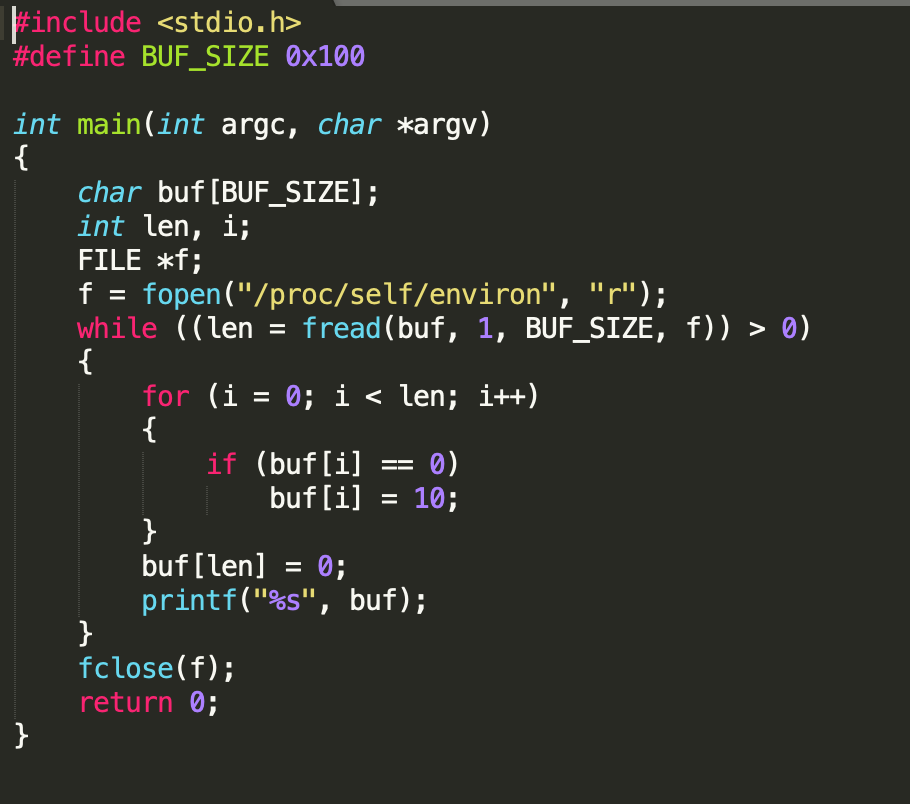
\includegraphics[scale = 1.0]{round.png}}
			\label{ris:round}
		\end{center}
	\end{figure}

	\newpage
	
	Результат выполнения программы:
	
	\begin{figure}[h!]
		\begin{center}
			{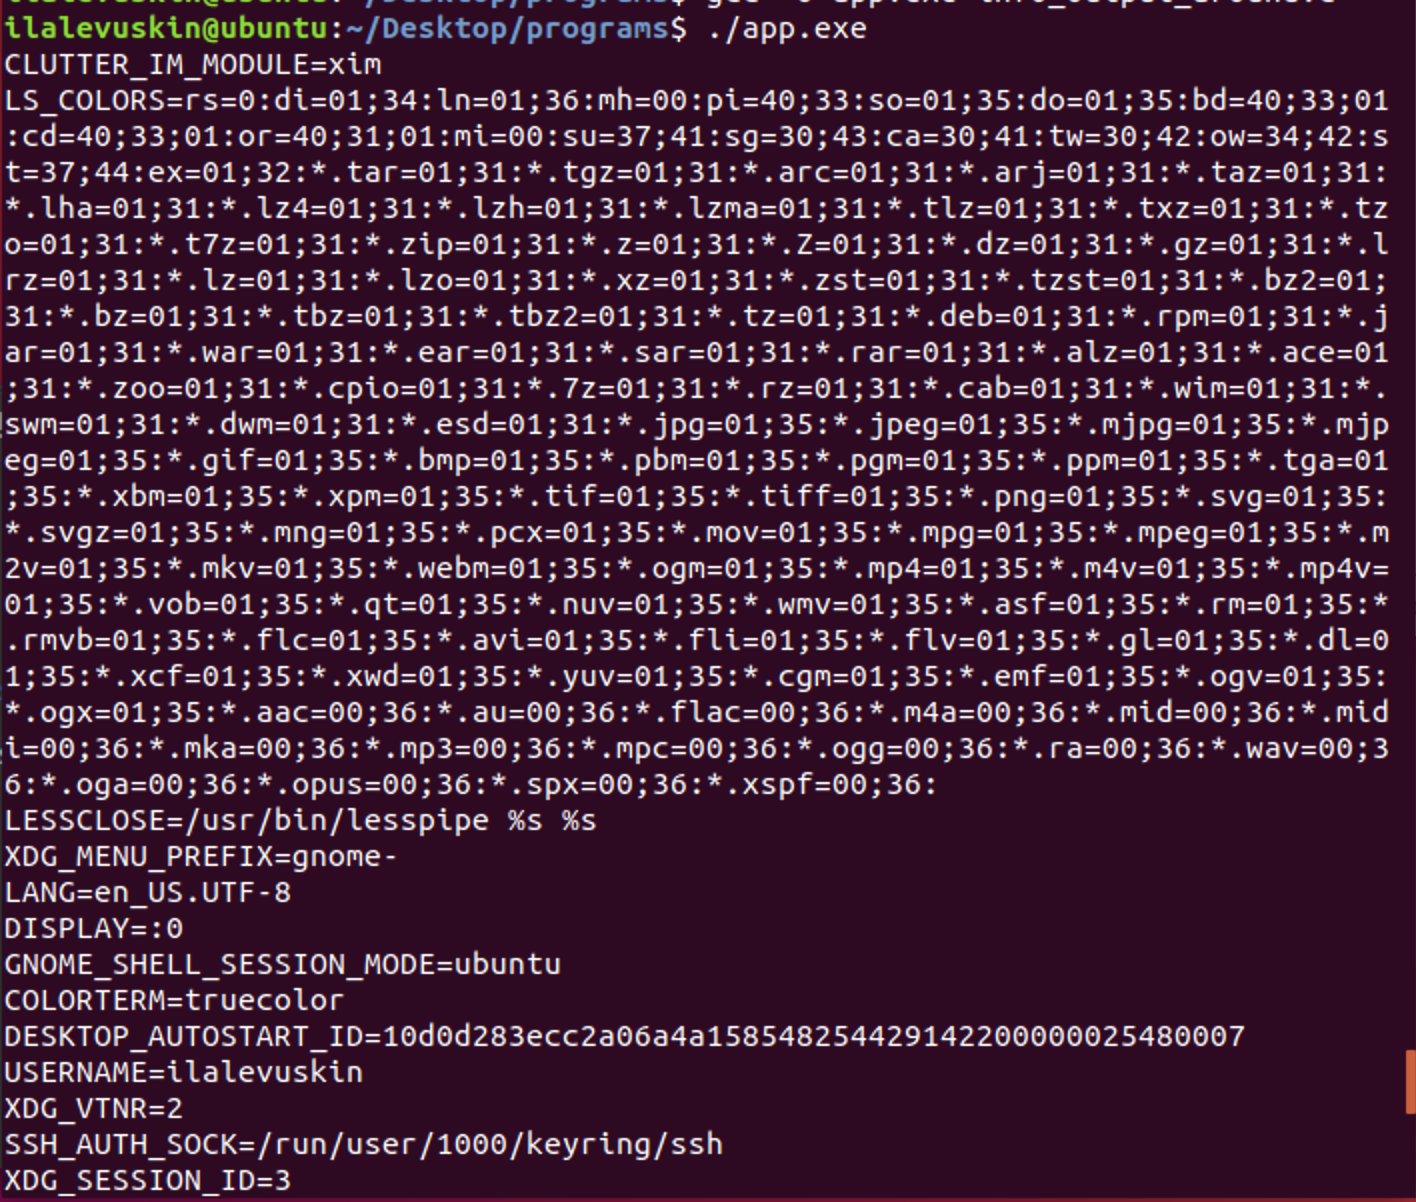
\includegraphics[scale = 0.6]{round1.png}}
			\label{ris:round1}
		\end{center}
	\end{figure}

	\begin{figure}[h!]
		\begin{center}
			{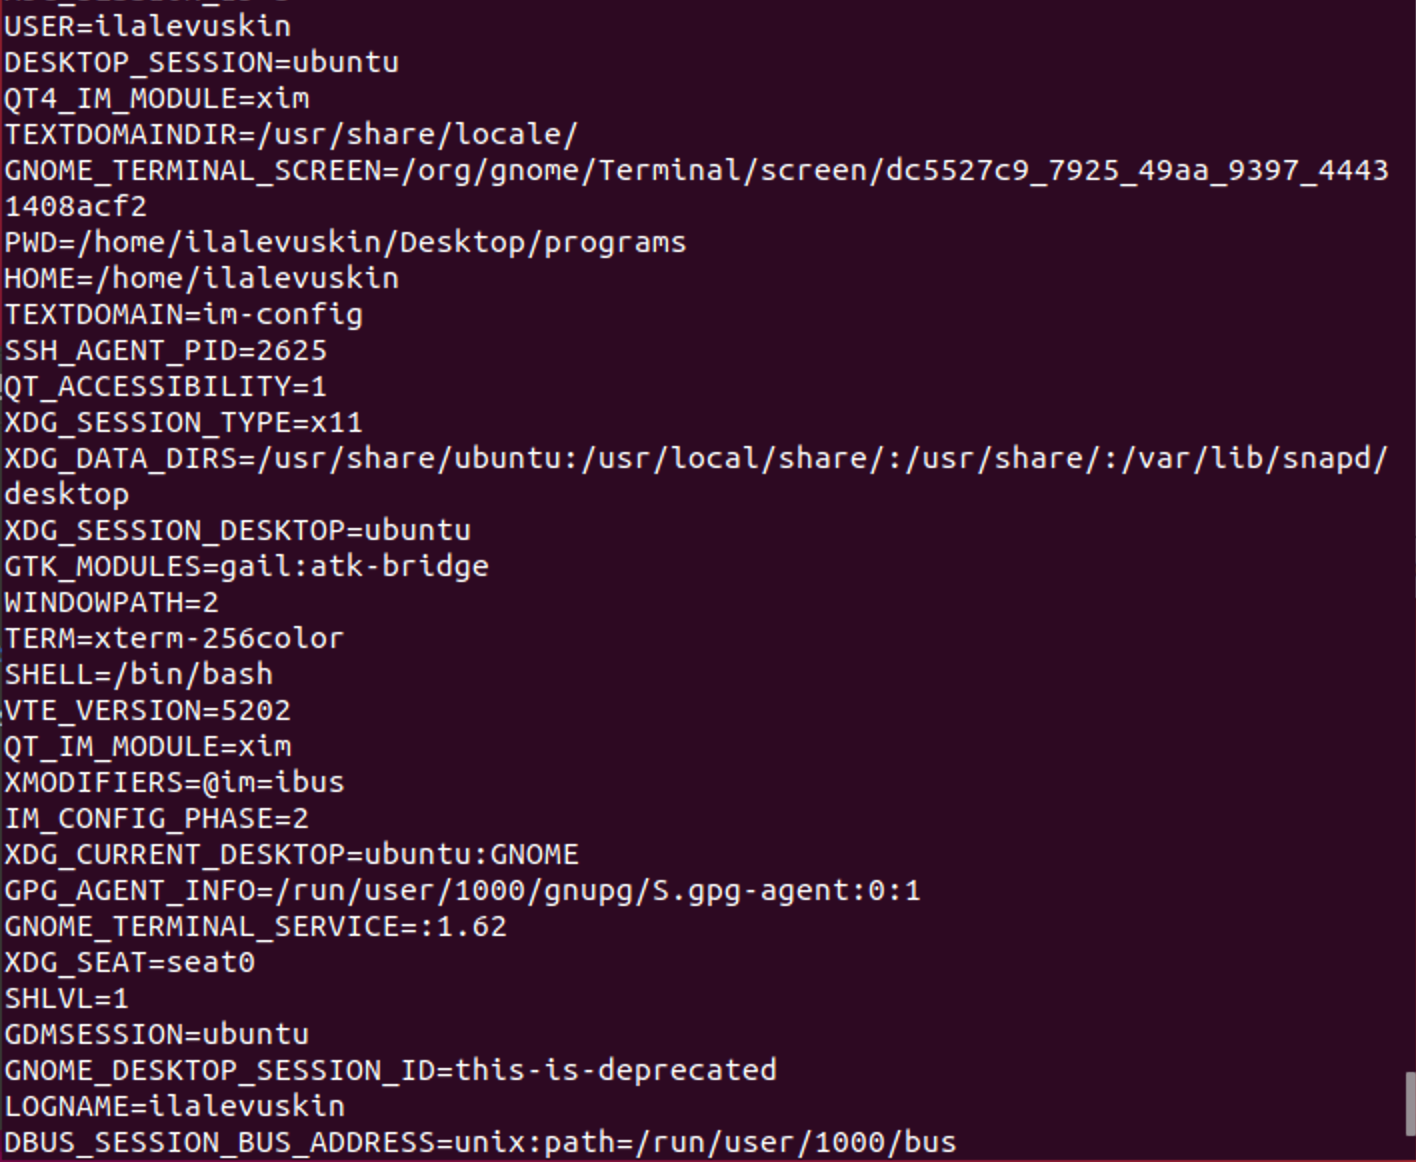
\includegraphics[scale = 0.55]{round2.png}}
			\label{ris:round2}
		\end{center}
	\end{figure}

	\newpage

	\begin{figure}[h!]
		\begin{center}
			{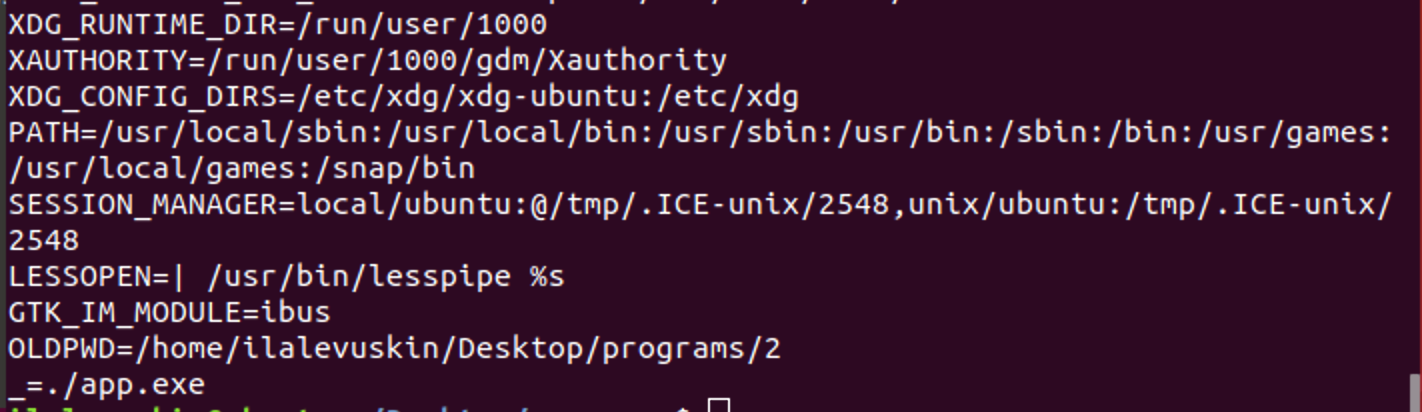
\includegraphics[scale = 0.7]{round3.png}}
			\label{ris:round3}
		\end{center}
	\end{figure}
	
	Окружение (environment) или среда — это набор пар
	ПЕРЕМЕННАЯ=ЗНАЧЕНИЕ, доступный каждому пользовательскому
	процессу. Иными словами, окружение — это набор переменных окружения.
	
	Некоторые переменные окружения:
	
	\begin{enumerate}
		\item LS\_COLORS=rs=0
		
		используется для определения цветов, с которыми будут выведены имена
		файлов при вызове ls.
		\item LESSCLOSE=/usr/bin/lesspipe \%s \%s
		
		LESSOPEN=| /usr/bin/lesspipe \%s
		
		определяют пре- и пост- обработчики файла, который открывается при вызове less.
		\item XDG\_MENU\_PREFIX=gnome-
		
		XDG\_VTNR=2
		
		XDG\_SESSION\_ID=3
		
		XDG\_SESSION\_TYPE=x11
		
		XDG\_SESSION\_DESKTOP=ubuntu
		
		XDG\_CURRENT\_DESKTOP=ubuntu:GNOME
		
		XDG\_RUNTIME\_DIR=/run/user/1000
		
		XDG\_CONFIG\_DIRS=/etc/xdg/xdg-ubuntu:/etc/xdg
		
		переменные, необходимые для вызова xdg-open, использующейся для
		открытия файла или URL в пользовательском приложении.
		\item LANG=en\_US.UTF-8
		
		язык и кодировка пользователя.
		\item DISPLAY=:0
		
		указывает приложениям, куда отобразить графический пользовательский
		интерфейс.
		\item GNOME\_SHELL\_SESSION\_MODE=ubuntu
		
		GNOME\_TERMINAL\_SCREEN=/org/gnome/Terminal/scree
		
		GNOME\_DESKTOP\_SESSION\_ID=this-is-deprecated
		
		GNOME\_TERMINAL\_SERVICE=:1.62
		
		переменные среды рабочего стола GNOME.
		\item COLORTERM=truecolor
		
		определяет поддержку 24-битного цвета.
		\item USER=ilalevushkin
		
		имя пользователя, от чьего имени запущен процесс.
		\item USERNAME=ilalevishkin
		
		имя пользователя, кто инициировал запуск процесса
		\item SSH\_AUTH\_SOCK=/run/user/1000/keyring/ssh
		
		путь к сокету, который агент использует для коммуникации с другими процессами.
		\item TEXTDOMAINDIR=/usr/share/locale/
		
		TEXTDOMAIN=im-config
		
		директория и имя объекта сообщения, получаемого при вызове gettext.
		\item PWD=/home/ilalevushkin/Desktop/programs
		
		путь к рабочей директории.
		\item HOME=/home/ilalevushkin
		
		путь к домашнему каталогу текущего пользователя.
		\item SSH\_AGENT\_PID=2625
		
		идентификатор процесса ssh-agent.
		\item TERM=xterm-256color
		
		тип запущенного терминала.
		\item SHELL=/bin/bash
		
		путь к предпочтительной оболочке командной строки.
		\item SHLVL=1
		
		уровень текущей командной оболочки.
		\item LOGNAME=ilalevushkin
		
		имя текущего пользователя.
		\item PATH=/usr/local/sbin:/usr/local/bin:/usr/sbin:/usr/bin:/sbin:/bin:/usr/games:/usr/local/games:/snap/bin
		
		список каталогов, в которых система ищет исполняемые файлы.
		\item \_=./app.exe - полная командная строка процесса.
	\end{enumerate}

	Ниже приведена программа для вывода информации, характеризующей состояние процесса:
	
	\begin{figure}[h!]
		\begin{center}
			{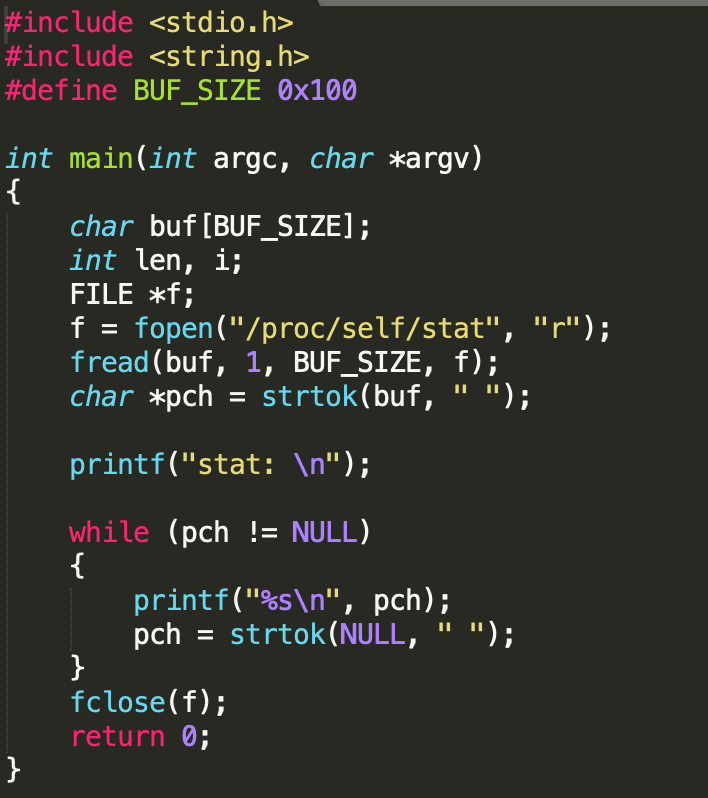
\includegraphics[scale = 0.7]{cond.png}}
			\label{ris:cond}
		\end{center}
	\end{figure}
	
	\newpage
	
	Результат выполнения программы:
	
	\begin{figure}[h!]
		\begin{center}
			{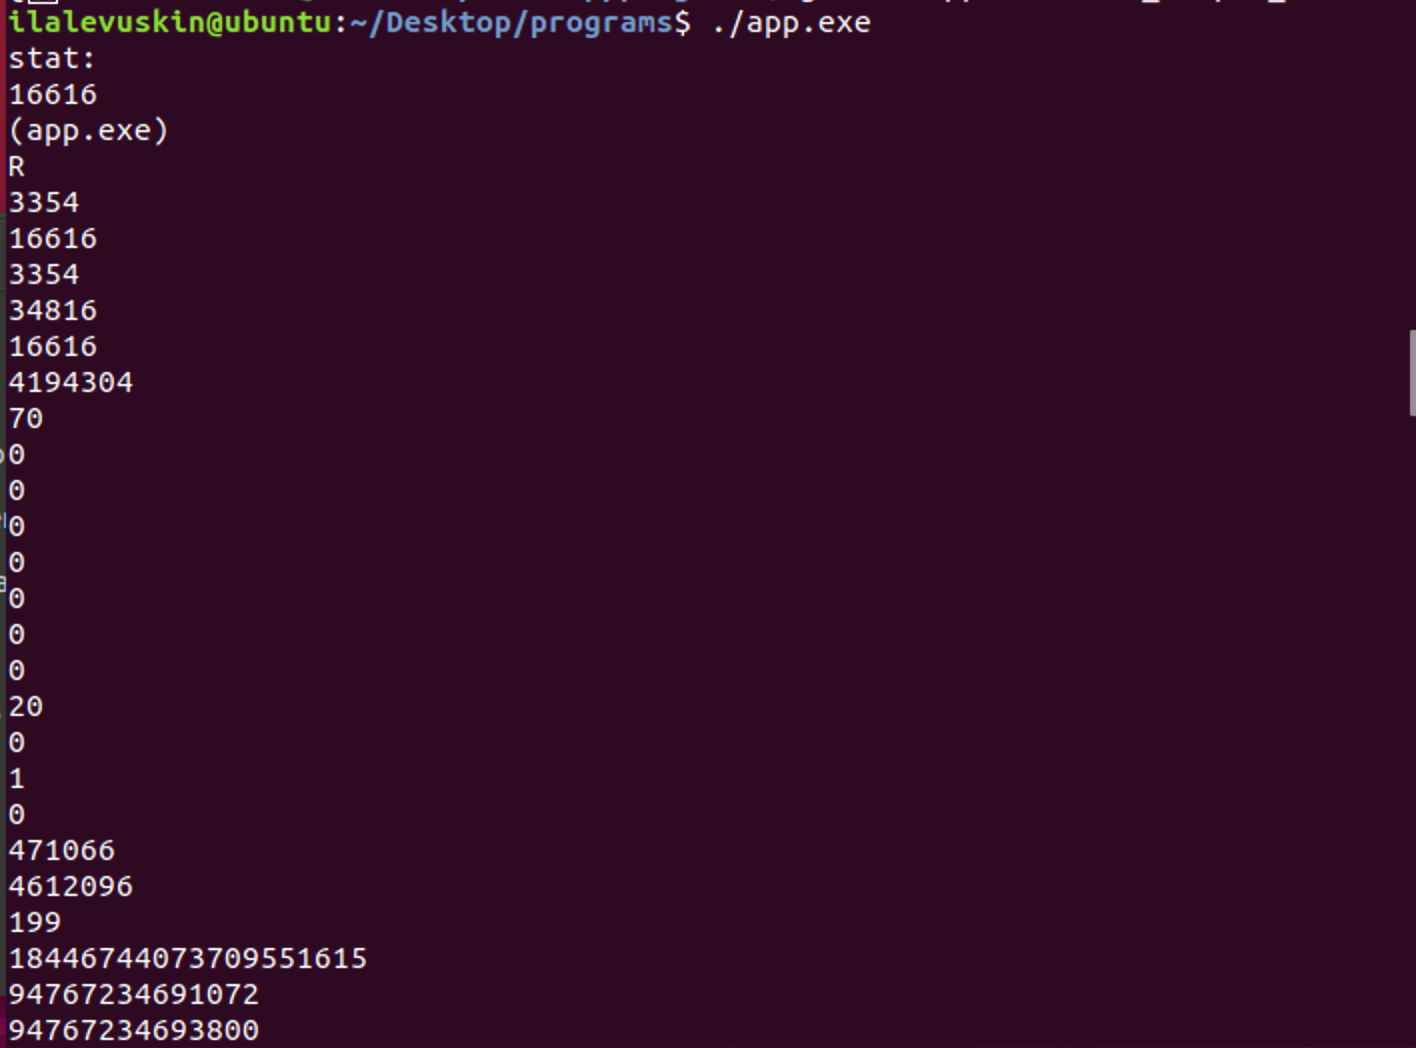
\includegraphics[scale = 0.7]{stat1.png}}
			\label{ris:stat1}
		\end{center}
	\end{figure}

	\begin{figure}[h!]
		\begin{center}
			{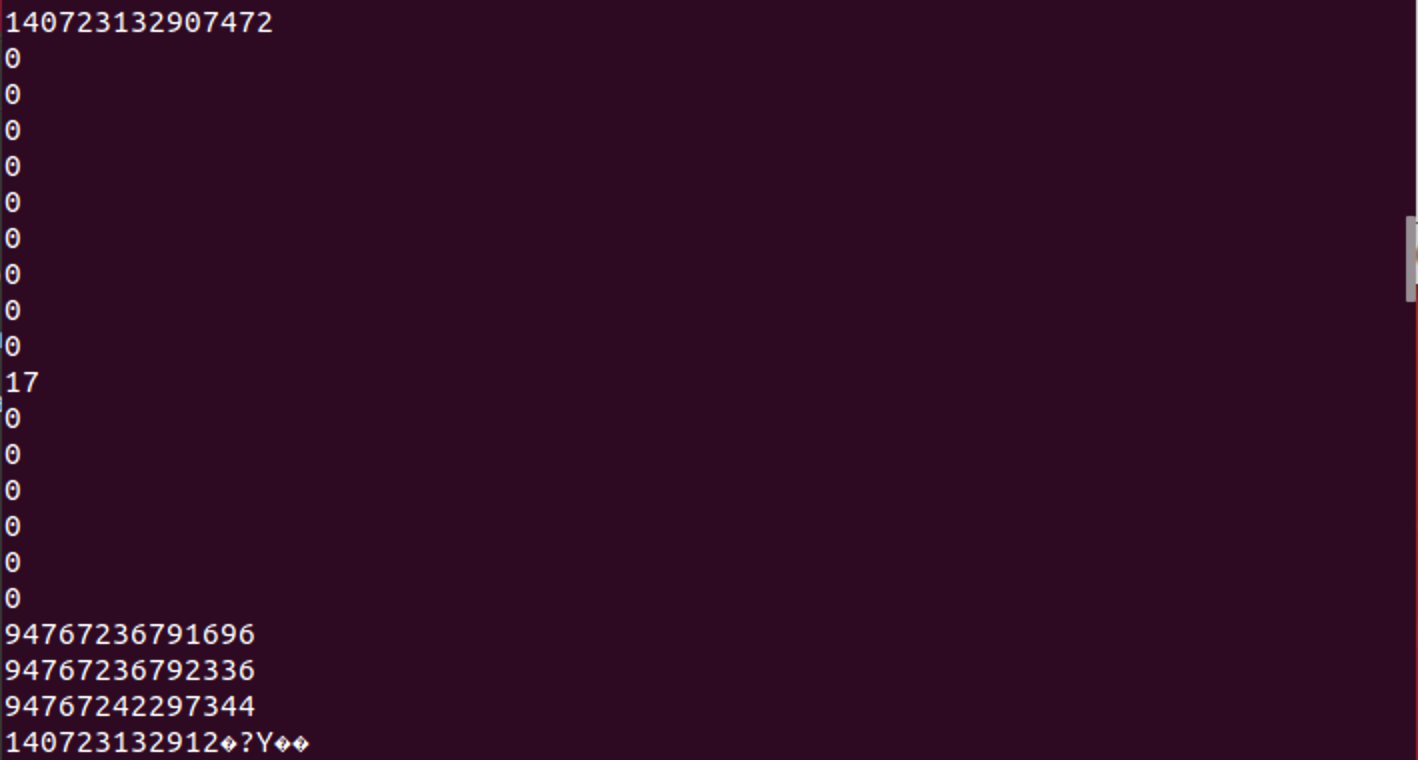
\includegraphics[scale = 0.7]{stat2.png}}
			\label{ris:stat2}
		\end{center}
	\end{figure}
	
	\newpage
	
	Содержимое файла /proc/[pid]/stat:
	
	\begin{enumerate}
		\item pid=16616 - уникальный идентификатор процесса.
		\item comm=(app.exe) - имя исполняемого файла в круглых скобках.
		\item state=R - состояние процесса.
		\item ppid=3354 - уникальный идентификатор процесса-предка.
		\item pgrp=16616 - уникальный идентификатор группы.
		\item session=3354 - уникальный идентификатор сессии.
		\item tty\_nr=34816 – управляющий терминал.
		\item tpgid=16616 – уникальный идентификатор группы управляющего терминала.
		\item flags=4194304 – флаги.
		\item minflt=70 - Количество незначительных сбоев, которые возникли при выполнении процесса, и которые не требуют загрузки страницы памяти с диска.
		\item cminflt=0 - количество незначительных сбоев, которые возникли при ожидании окончания работы процессов-потомков.
		\item majflt=0 - количество значительных сбоев, которые возникли при работе процесса, и которые потребовали загрузки страницы памяти с диска.
		\item cmajflt=0 - количество значительных сбоев, которые возникли при ожидании окончания работы процессов-потомков.
		\item utime=0 - количество тиков, которые данный процесс провел в режиме пользователя.
		\item stime=0 - количество тиков, которые данный процесс провел в режиме ядра.
		\item cutime=0 - количество тиков, которые процесс, ожидающий завершения процессов-потомков, провёл в режиме пользователя.
		\item cstime=0 - количество тиков, которые процесс, ожидающий завершения процессов-потомков, провёл в режиме ядра.
		\item priority=20 – для процессов реального времени это отрицательный приоритет планирования минус один, то есть число в диапазоне от -2 до -100, соответствующее приоритетам в реальном времени от 1 до 99. Для остальных процессов это необработанное значение nice, представленное в ядре. Ядро хранит значения nice в виде чисел в диапазоне от 0 (высокий) до 39 (низкий), соответствующих видимому пользователю диапазону от -20 до 19.
		\item nice=0 - значение для nice в диапазоне от 19 (наиболее низкий приоритет) до -20 (наивысший приоритет).
		\item num\_threads=1 – число потоков в данном процессе.
		\item itrealvalue=0 – количество мигов до того, как следующий SIGALARM будет послан процессу интервальным таймером. С ядра версии 2.6.17 больше не поддерживается и установлено в 0.
		\item starttime=471066 - время в тиках запуска процесса после начальной загрузки системы.
		\item vsize=4612096 - размер виртуальной памяти в байтах.
		\item rss=199 - резидентный размер: количество страниц, которые занимает процесс в памяти. Это те страницы, которые заняты кодом, данными и пространством стека.
		
		Сюда не включаются страницы, которые не были загружены по требованию или которые находятся в своппинге.
		\item rsslim=18446744073709551615 - текущий лимит в байтах на резидентный размер процесса.
		\item startcode=94767234691072 - адрес, выше которого может выполняться код программы.
		\item endcode=94767234693800 - адрес, ниже которого может выполняться код программ.
		\item startstack=140723132907472 - адрес начала стека.
		\item kstkesp=0 - текущее значение ESP (указателя стека).
		\item kstkeip=0 - текущее значение EIP (указатель команд).
		\item signal=0 - битовая карта ожидающих сигналов. Устарела, потому что не предоставляет информацию о сигналах реального времени, необходимо использовать /proc/[pid]/status.
		\item blocked=0 - битовая карта блокируемых сигналов. Устарела, потому что не предоставляет информацию о сигналах реального времени, необходимо использовать /proc/[pid]/status.
		\item sigignore=0 - битовая карта игнорируемых сигналов. Устарела, потому что не предоставляет информацию о сигналах реального времени, необходимо
		использовать /proc/[pid]/status.
		\item sigcatch=0 - битовая карта перехватываемых сигналов. Устарела, потому что не предоставляет информацию о сигналах реального времени, необходимо
		использовать /proc/[pid]/status.
		\item wchan=0 - "канал", в котором ожидает процесс.
		\item nswap=0 - количество страниц на своппинге (не обслуживается).
		\item сnswap=0 - суммарное nswap для процессов-потомков (не обслуживается).
		\item exit\_signal=17 - сигнал, который будет послан предку, когда процесс завершится.
		\item processor=0 - номер процессора, на котором последний раз выполнялся процесс.
		\item rt\_priority=0 - приоритет планирования реального времени, число в диапазоне от
		1 до 99 для процессов реального времени, 0 для остальных.
		\item policy=0 - политика планирования.
		\item delayacct\_blkio\_ticks=0 - суммарные задержки ввода/вывода в тиках.
		\item guest\_time=0 – гостевое время процесса (время, потраченное на выполнение
		виртуального процессора на гостевой операционной системе) в тиках.
		\item cguest\_time=0 - гостевое время для потомков процесса в тиках.
		\item start\_data=94767236791696 - адрес, выше которого размещаются
		инициализированные и неинициализированные (BSS) данные программы.
		\item end\_data=94767236791696 - адрес, ниже которого размещаются
		инициализированные и неинициализированные (BSS) данные программы.
		\item start\_brk=94767242297344 - адрес, выше которого куча программы может быть
		расширена с использованием brk().
		\item arg\_start=140723132912 - адрес, выше которого размещаются аргументы
		командной строки (argv).
	\end{enumerate}
	
	\newpage
	
	Листинг ссылка программы для вывода содержания директории fd:
	
	\begin{figure}[h!]
		\begin{center}
			{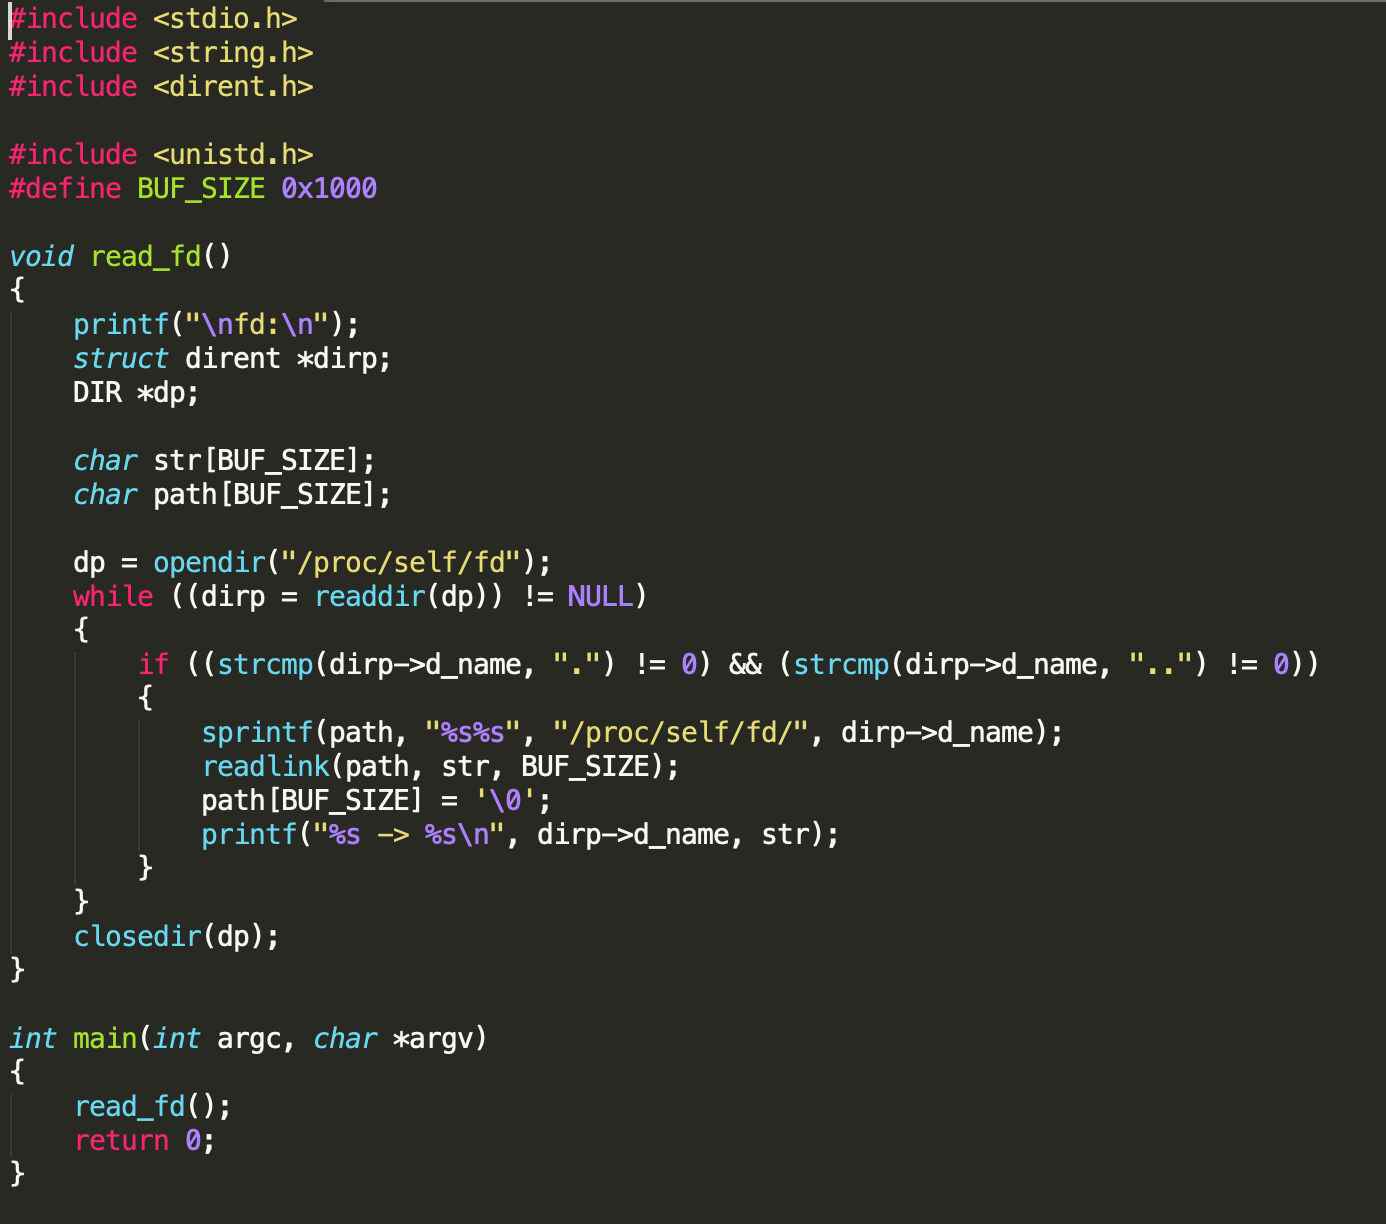
\includegraphics[scale = 0.7]{fd1.png}}
			\label{ris:fd1}
		\end{center}
	\end{figure}
	
	Результат выполнения программы
	
	\begin{figure}[h!]
		\begin{center}
			{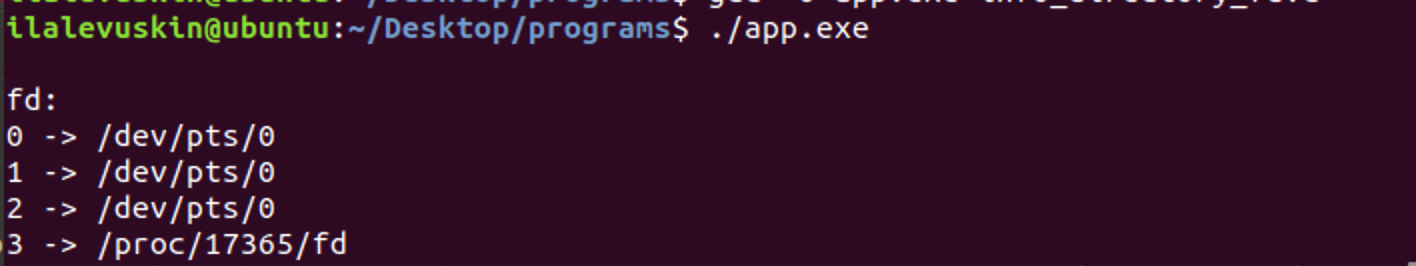
\includegraphics[scale = 0.7]{fd.png}}
			\label{ris:fd}
		\end{center}
	\end{figure}
	
	\newpage
	
	Ниже приведена программа для вывода содержания директории cmdline:
	
	\begin{figure}[h!]
		\begin{center}
			{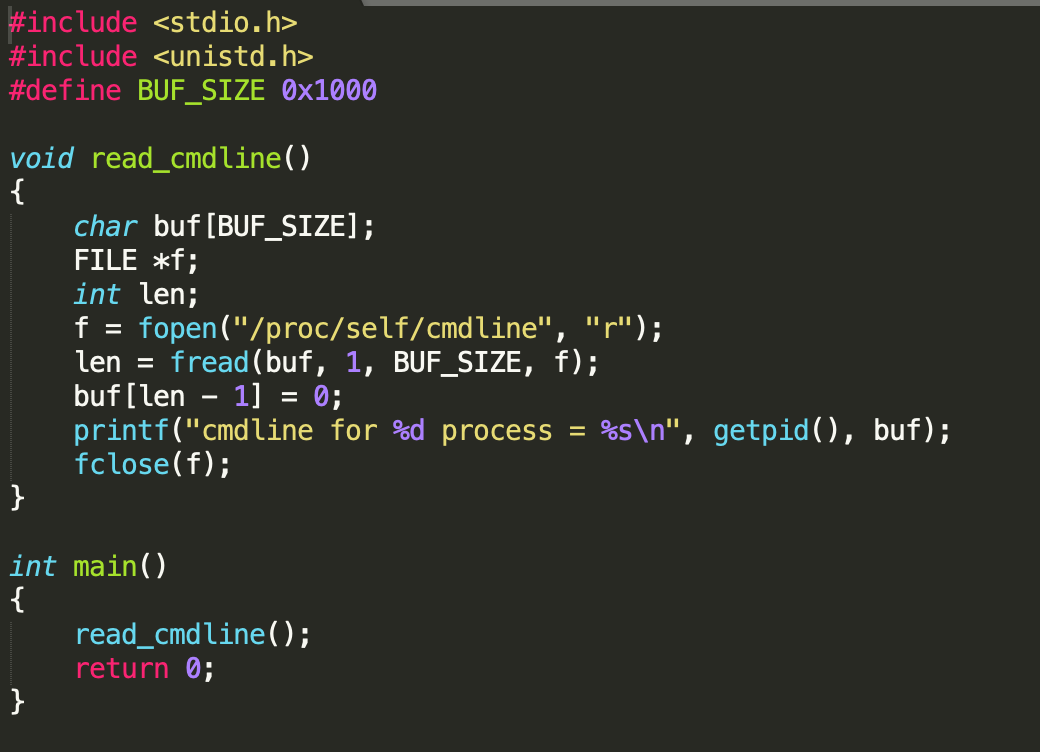
\includegraphics[scale = 0.7]{cmdline1.png}}
			\label{ris:cmdline1}
		\end{center}
	\end{figure}
	
	Результат выполнения программы:
	
	\begin{figure}[h!]
		\begin{center}
			{
\includegraphics[scale = 0.7]{cmdline.png}}
			\label{ris:cmdline}
		\end{center}
	\end{figure}
	
	\section*{Задание 2.}
	
	{\bf Написать загружаемый модуль ядра, создать файл в файловой системе proc,
		sysmlink, subdir. Используя соответствующие функции передать данные из
		пространства пользователя в пространство ядра (введенные данные вывести
		в файл ядра) и из пространства ядра в пространство пользователя.
		Продемонстрировать это.}
	
	\newpage
	
	Листинг программы:
	
	\begin{figure}[h!]
		\begin{center}
			{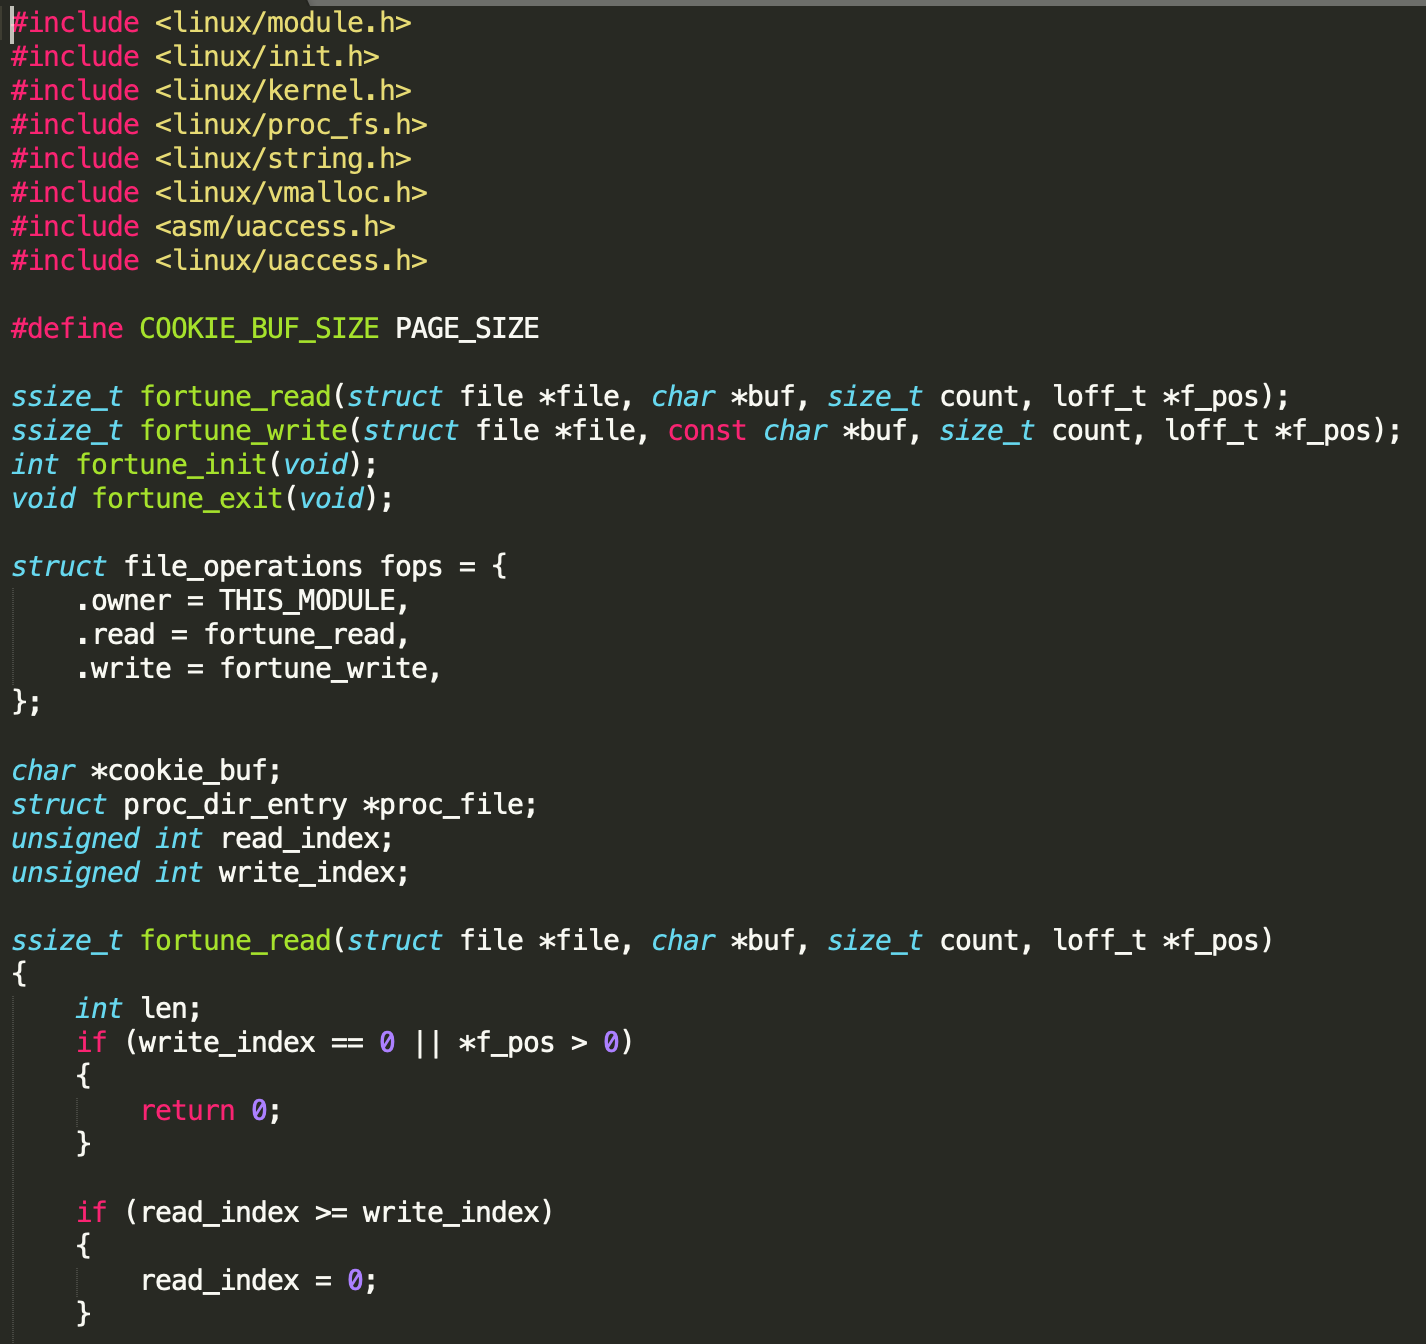
\includegraphics[scale = 0.7]{fortune1.png}}
			\label{ris:fortune1}
		\end{center}
	\end{figure}

	\newpage

	\begin{figure}[h!]
		\begin{center}
			{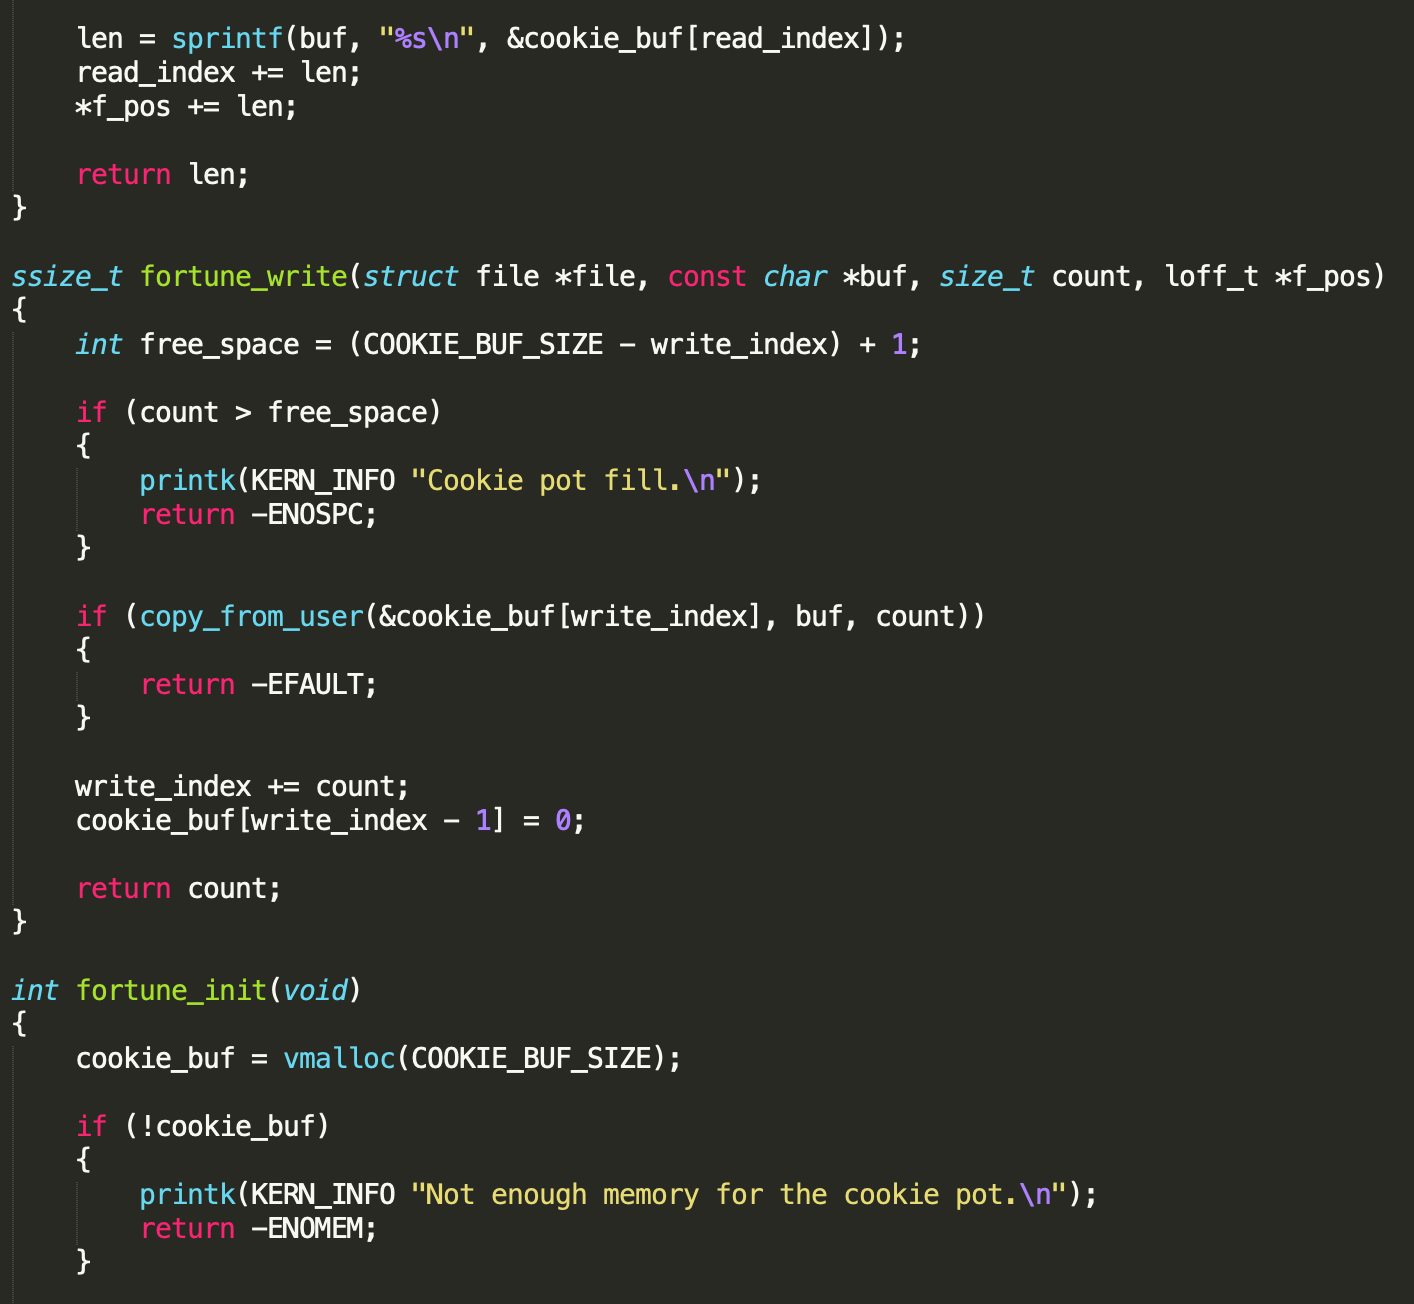
\includegraphics[scale = 0.7]{fortune2.png}}
			\label{ris:fortune2}
		\end{center}
	\end{figure}

	\newpage

	\begin{figure}[h!]
		\begin{center}
			{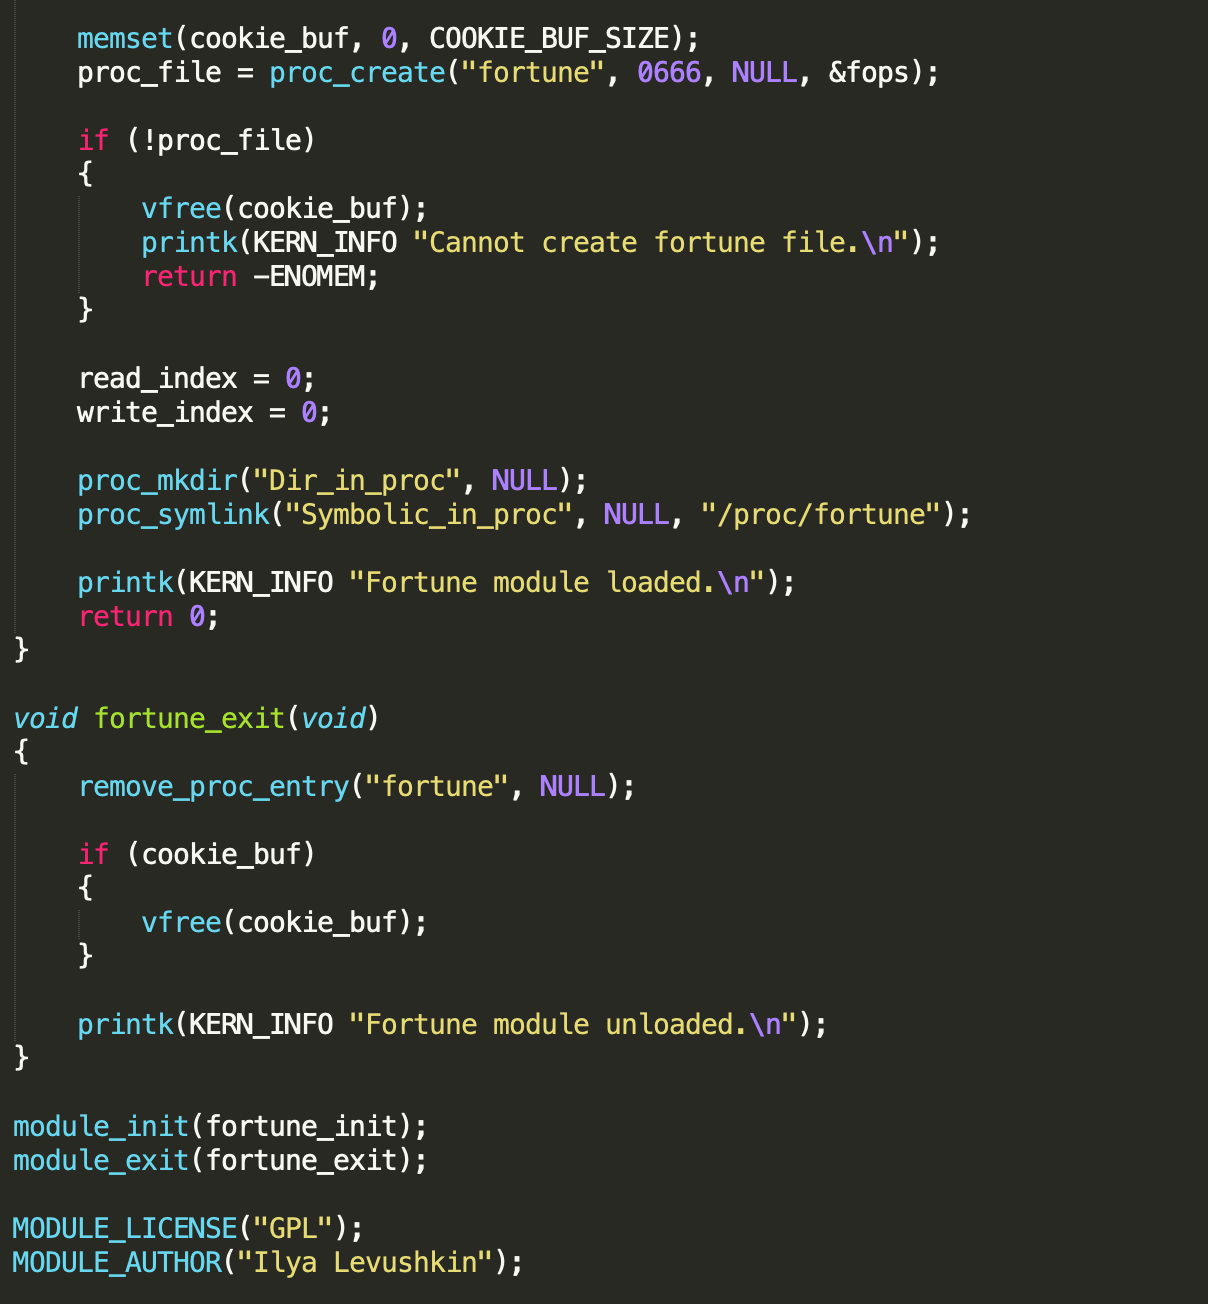
\includegraphics[scale = 0.7]{fortune3.png}}
			\label{ris:fortune3}
		\end{center}
	\end{figure}
	
	\newpage
	
	Скриншоты:
	
	\begin{figure}[h!]
		\begin{center}
			{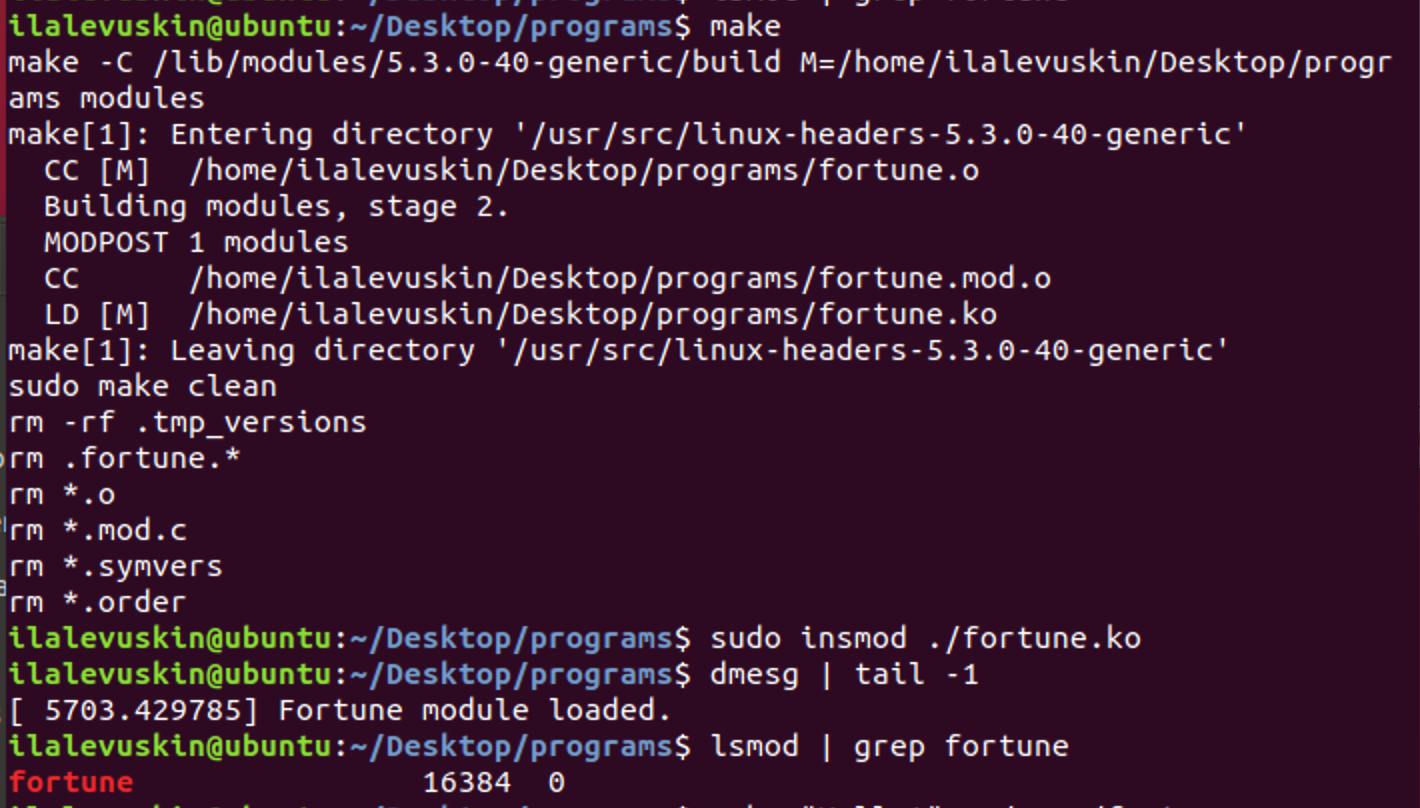
\includegraphics[scale = 0.7]{make.png}}
			\label{ris:make}
		\end{center}
	\end{figure}

	\begin{figure}[h!]
		\begin{center}
			{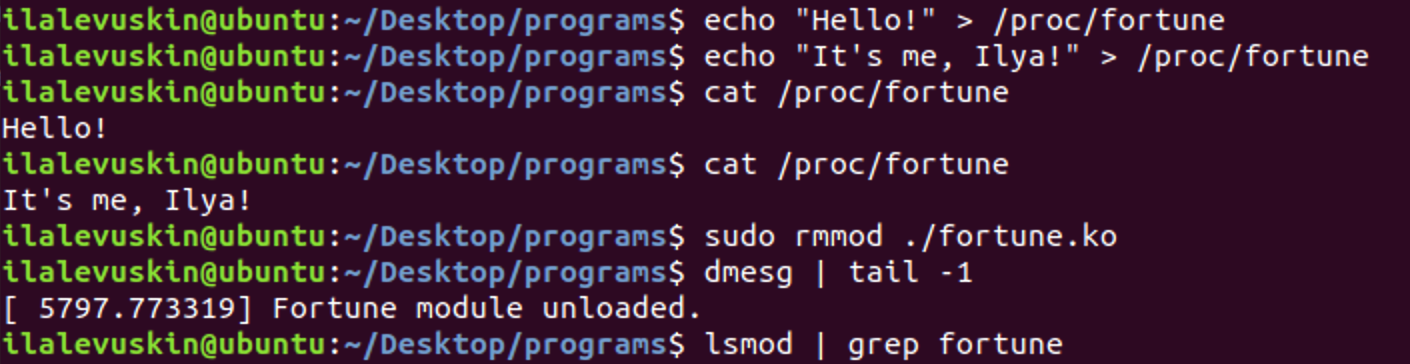
\includegraphics[scale = 0.7]{hello.png}}
			\label{ris:hello}
		\end{center}
	\end{figure}

	\begin{figure}[h!]
		\begin{center}
			{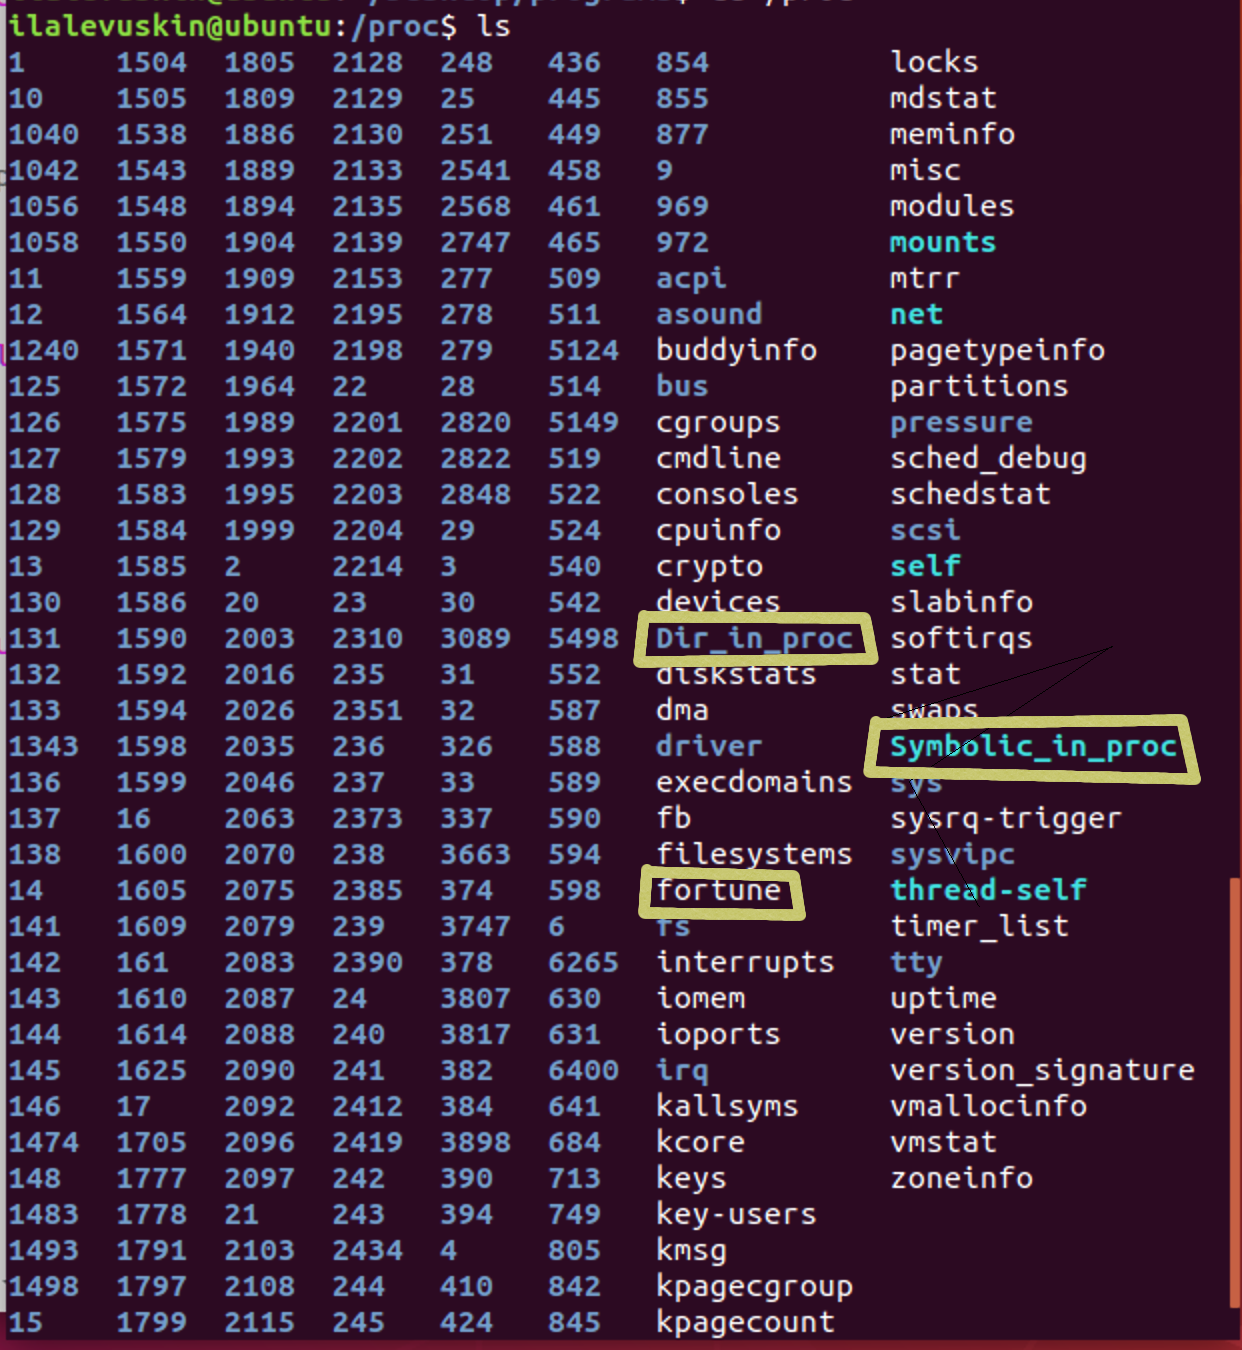
\includegraphics[scale = 0.7]{example.png}}
			\label{ris:example}
		\end{center}
	\caption{Созданные файл, поддиректория и символьная ссылка в директории /proc}
	\end{figure}
			
\end{document}